% Presentation on keg
%
\documentclass{beamer}
%\documentclass[handout]{beamer}
%\usepackage{beamerthemeshadow}
\usetheme{Warsaw}
\usepackage{pgf}
\usepackage{multimedia}

%\pgfdeclareimage[interpolate=true,height=7cm]{faktorial}{faktorial}

\author{Michal Kov\'{a}\v{c}}
\title{User oriented language for powerful data mining with Ferda}
\date{\today}

\begin{document}
\frame{\titlepage}

\section{Introduction}
\subsection{Table of contents}
\frame{
	\frametitle{Table of contents part 1/2}
	\tableofcontents[sections={1-2},pausesections]
}

\frame{
	\frametitle{Table of contents part 2/2}
	\tableofcontents[sections={3-4},pausesections]
}

\subsection{What is Ferda Data Miner?}
\begin{frame}
	\frametitle{Ferda}
	\begin{block}{What is Ferda?}
		\begin{itemize}[<+->]
			\item User oriented application
			\item For specification of tasks, execution and result browsing
			\item Works with boxes
			\item Ferda Data Miner = Ferda + boxes for data mining
		\end{itemize}
	\end{block}
	\begin{block}<+->{History}
		\begin{itemize}[<+->]
			\item LISp-Miner not so user frienly
			\item Software project at MFF
			\item Master theses
		\end{itemize}
	\end{block}
\end{frame}

\begin{frame}
	\frametitle{Screenshot}
	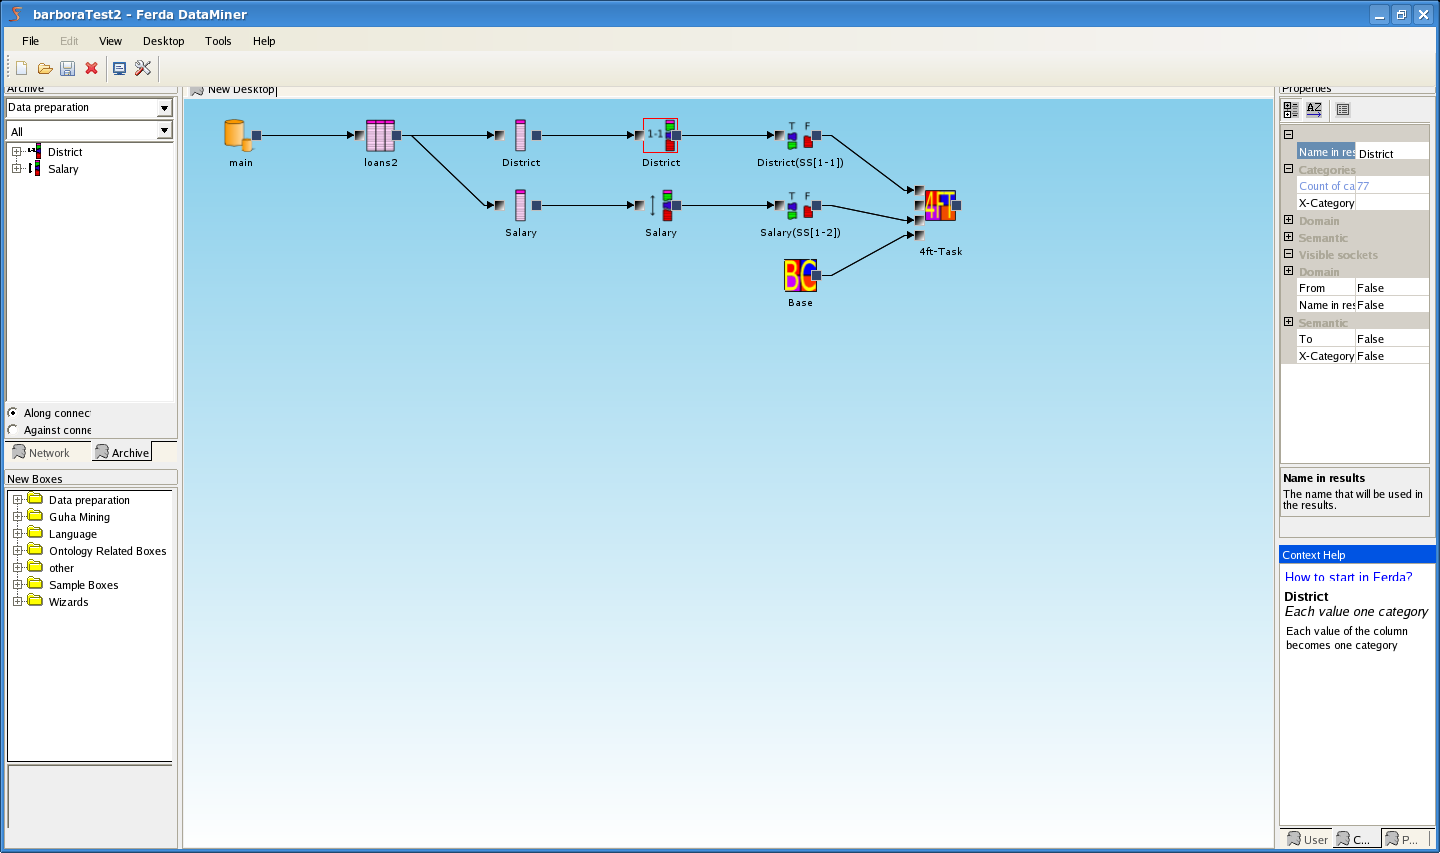
\includegraphics[width=10.8cm]{ferda}
\end{frame}

\subsection{Ferda as programming language}
\begin{frame}
	\frametitle{Ferda as programming language}
	\begin{block}<+->{Box as function}
		\begin{itemize}[<+->]
			\item Box consists of functions
			\item Sockets are parameters of these functions
			\item Property is also socket
				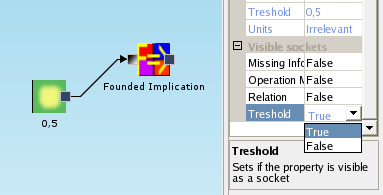
\includegraphics[width=7cm]{property_as_socket}
		\end{itemize}
	\end{block}	
\end{frame}

\subsection{What is missing? What should be done?}
\begin{frame}
	\frametitle{What is missing?}
	\begin{block}{What is missing?}
		\begin{itemize}[<+->]
			\item Moving work from one project to another
			\item Basic math boxes
			\item Recursion
			\item Other language boxes
			\item Ferda specific language boxes
			\item Data mining specific boxes for user programming
		\end{itemize}
	\end{block}
\end{frame}

\section{New functionality in Ferda}
\subsection{Network archive}
\begin{frame}
	\frametitle{Network archive}
	\begin{block}{What is network archive?}
		\begin{itemize}[<+->]
			\item New place where user can store connection
			\item Independent on project
			\item One network archive can be accessed from more computers
			\item Way how to move connections from one project to another
		\end{itemize}
	\end{block}
\end{frame}

\begin{frame}
	\frametitle{Movie -- network archive}
	\movie[externalviewer]{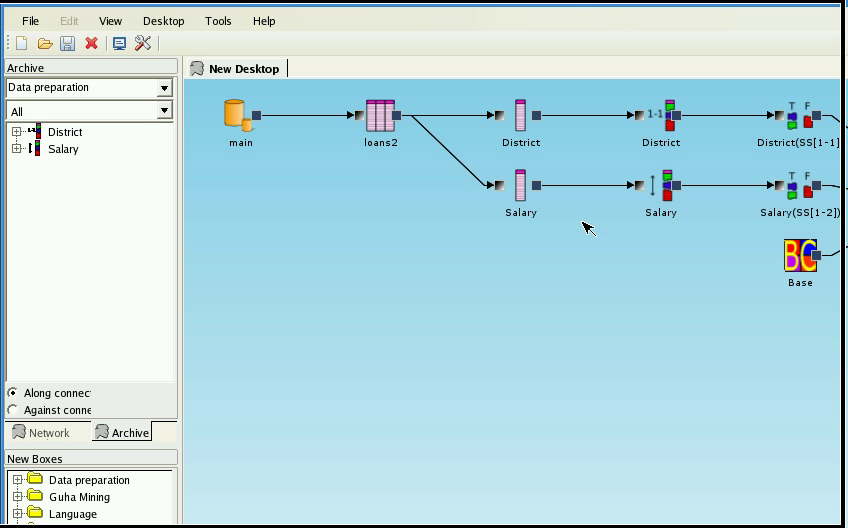
\includegraphics[width=10.8cm]{networkArchive1}}{networkArchive.ogg}
\end{frame}

\begin{frame}
	\frametitle{Screenshot -- add a connection to the network archive}
	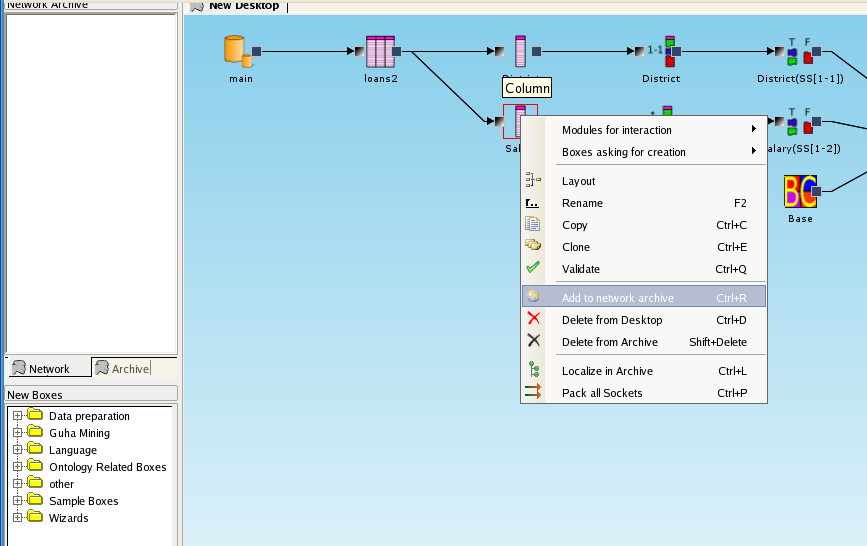
\includegraphics[width=10.8cm]{add_to_network_archive}
\end{frame}

\begin{frame}
	\frametitle{Screenshot -- set a name of box in the network archive}
	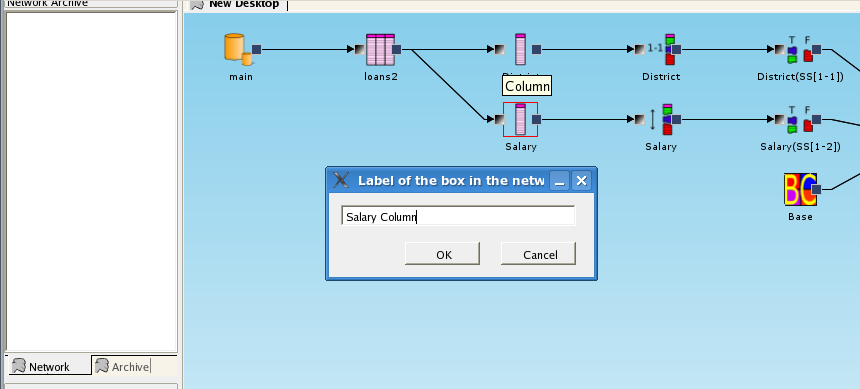
\includegraphics[width=10.8cm]{set_name_of_box_in_network_archive}
\end{frame}

\begin{frame}
	\frametitle{Screenshot -- new box added to the network archive}
	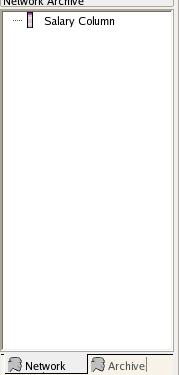
\includegraphics[height=7cm]{network_archive_box_added}
\end{frame}

\begin{frame}
	\frametitle{Screenshot -- drop box to a desktop from the n. archive}
	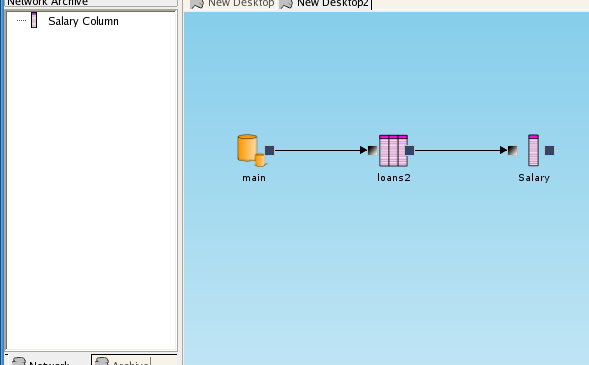
\includegraphics[width=10.8cm]{network_archive_drop_to_desktop}
\end{frame}

\begin{frame}
	\frametitle{Screenshot -- remove box from the network archive}
	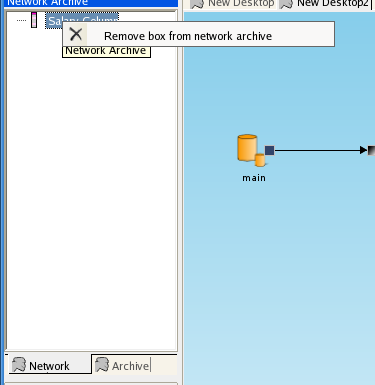
\includegraphics[height=7cm]{network_archive_remove_box}
\end{frame}

\subsection{Boxes for math}
\begin{frame}
	\frametitle{Movie -- Binary operation}
	\movie[externalviewer]{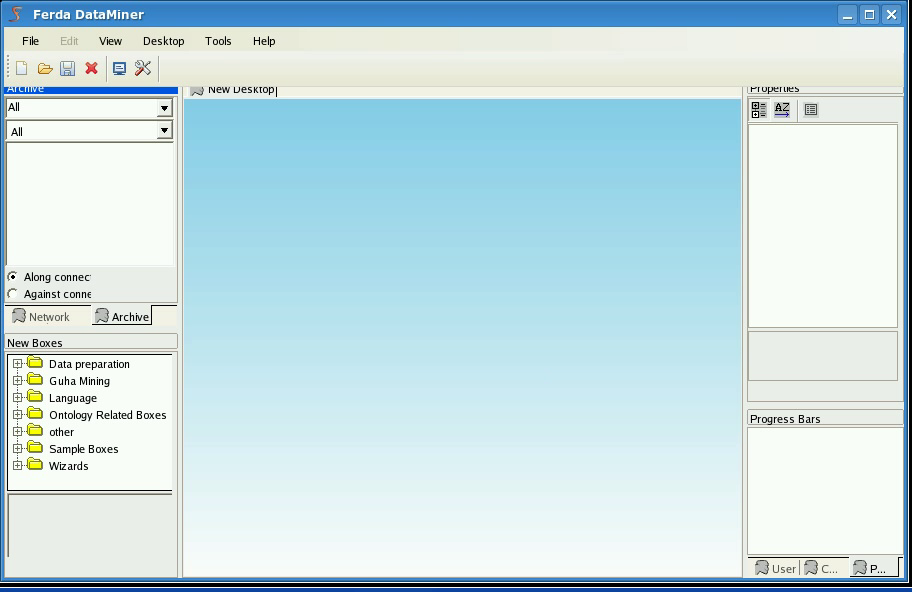
\includegraphics[width=10.8cm]{binaryOperation1.png}}{binaryOperation.ogg}
\end{frame}

\begin{frame}
	\frametitle{Binary operation}
	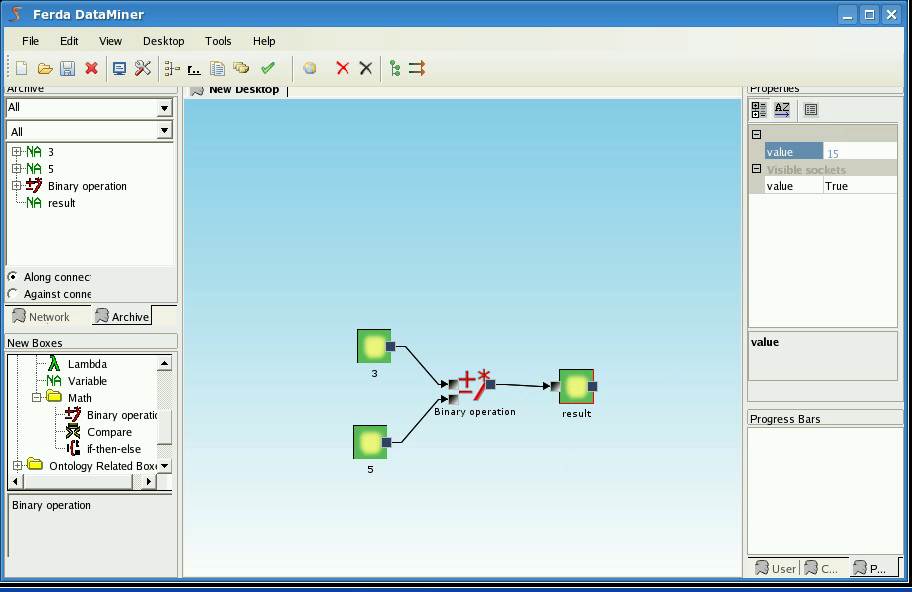
\includegraphics[width=10.8cm]{binaryOperation2.png}
\end{frame}

\begin{frame}
	\frametitle{Movie -- Comparision}
	\movie[externalviewer]{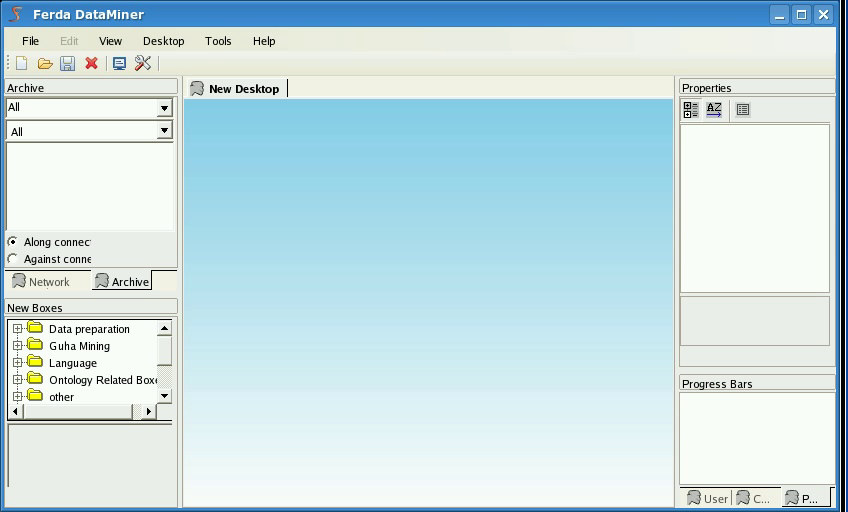
\includegraphics[width=10.8cm]{compare1.png}}{compare.ogg}
\end{frame}

\begin{frame}
	\frametitle{Comparision}
	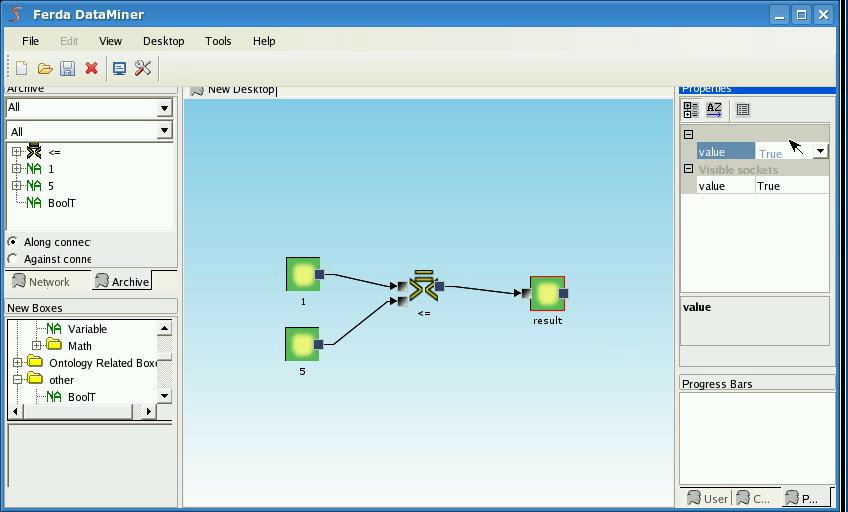
\includegraphics[width=10.8cm]{compare2.png}
\end{frame}

\begin{frame}
	\frametitle{Movie -- If expression}
	\movie[externalviewer]{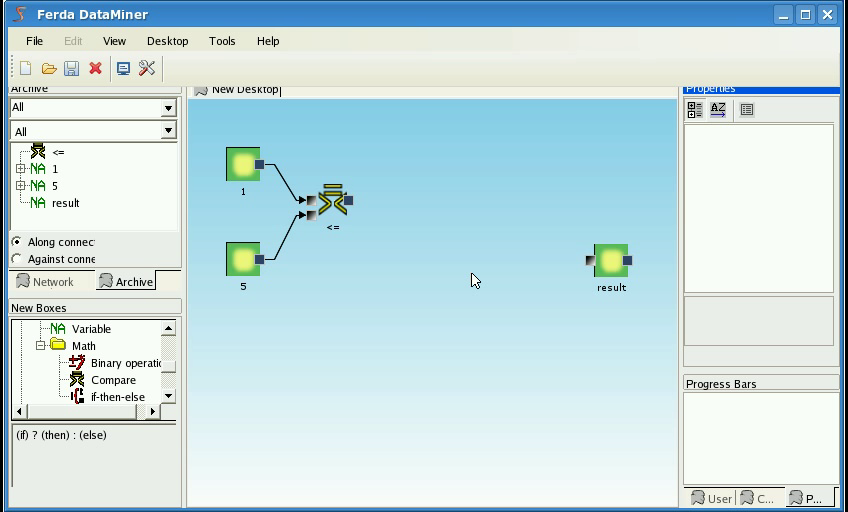
\includegraphics[width=10.8cm]{ifthenelse1.png}}{ifthenelse.ogg}
\end{frame}

\begin{frame}
	\frametitle{If expressions}
	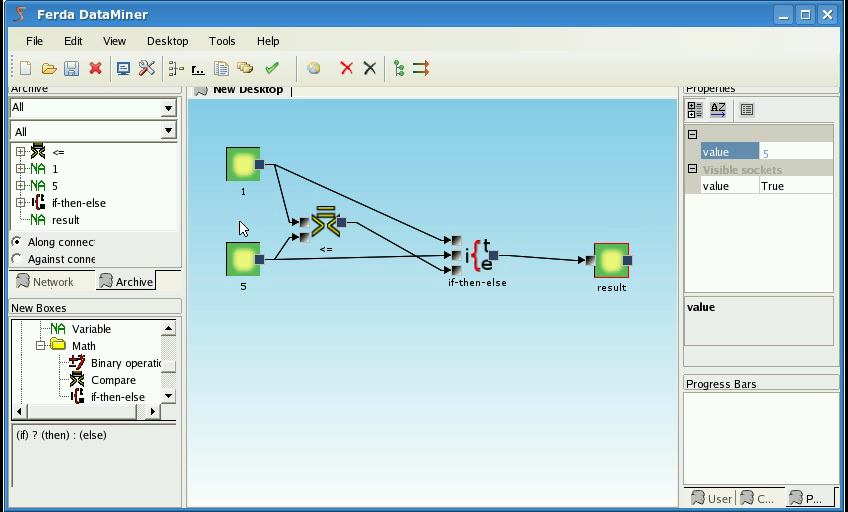
\includegraphics[width=10.8cm]{ifthenelse2.png}
\end{frame}

\subsection{Lambda expression}
\begin{frame}[fragile]
	\frametitle{Lambda expression}
	\begin{block}{Basic facts}
		\begin{itemize}[<+->]
			\item From lambda calculus $(\lambda x.(1+x))(9)$
			\item Basics of functional programming
		\end{itemize}
	\end{block}
	\begin{block}<+->{Lambda in C\# 3}
\begin{verbatim}
public delegate int function(int x);

public static void Main(string[] args)
{
  function plusOne = x => 1 + x;
  var a = plusOne(9);
  System.Console.WriteLine(a);
}
\end{verbatim}
	\end{block}	
\end{frame}

\begin{frame}[fragile]
	\frametitle{Lambda expression}
	\framesubtitle{Other languages}
	\begin{block}<+->{Lambda in F\#}
\begin{verbatim}
let onePlus x = 1 + x
do printf "%s" (onePlus(9)) 
\end{verbatim}
	\end{block}	
	\begin{block}<+->{Lambda in Python}
\begin{verbatim}
plusOne = lambda x: 1 + x
print plusOne(9)
\end{verbatim}
	\end{block}	
\end{frame}

\begin{frame}
	\frametitle{Movie -- Lambda basics in Ferda}
	\movie[externalviewer]{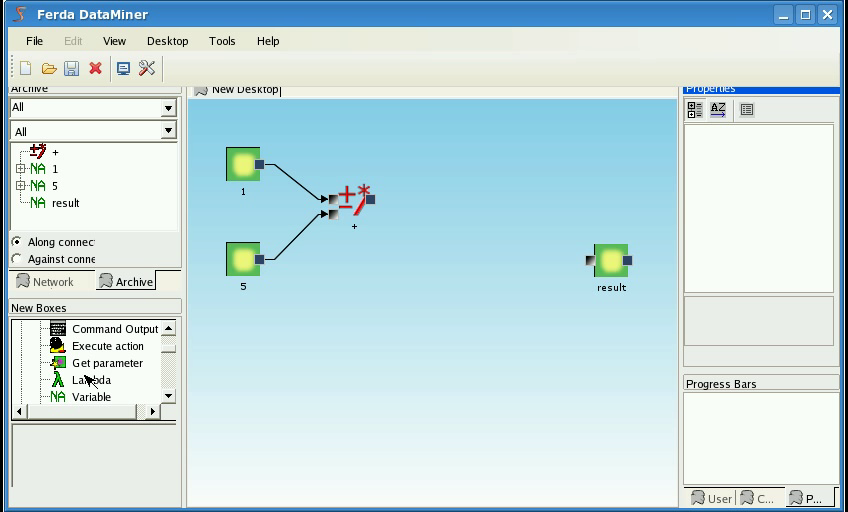
\includegraphics[width=10.8cm]{lambdaBasic1.png}}{lambdaBasic.ogg}
\end{frame}

\begin{frame}
	\frametitle{Basic use in Ferda}
	\framesubtitle{Lambda without parameters}

	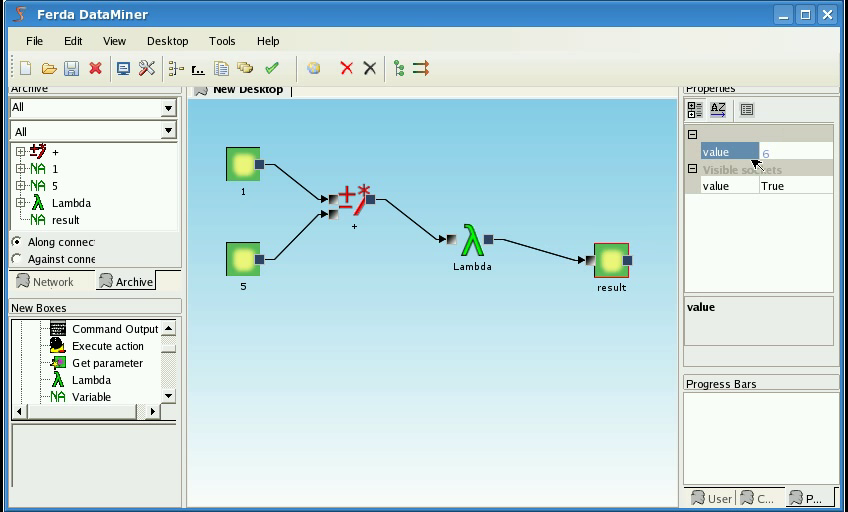
\includegraphics[width=10.8cm]{lambdaBasic2.png}
\end{frame}

\begin{frame}
	\frametitle{Basic use in Ferda}
	\framesubtitle{One constant parameter specified}
	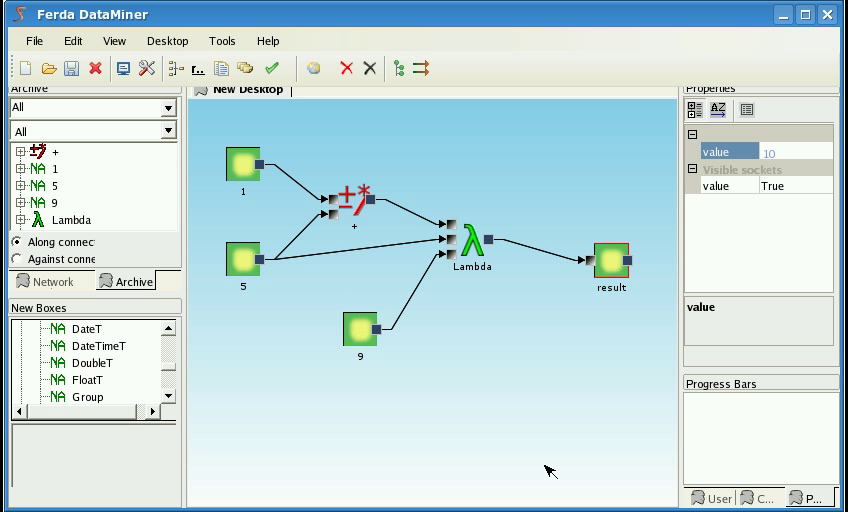
\includegraphics[width=10.8cm]{lambdaBasic3.png}
\end{frame}

\begin{frame}
	\frametitle{Implementation of lambda}
	\framesubtitle{How it really works}
	\begin{block}{Algoritm}
		\begin{itemize}[<+->]
			\item Values of variables are cloned (whole subtree)
			\item Main function is cloned with substitution and returned
		\end{itemize}
	\end{block}
\end{frame}

\begin{frame}[fragile]
	\frametitle{Factorial in C\#}
	\framesubtitle{Structural version}

	\begin{block}{First version of factorial}
\begin{verbatim}
public static int Factorial(int x)
{
  if (x == 0)
  {
    return 1;
  }
  else
  {
    return x * Factorial(x - 1);
  }
}
\end{verbatim}
	\end{block}
\end{frame}

\begin{frame}[fragile]
	\frametitle{Factorial in C\#}
	\framesubtitle{Expresion version}

	\begin{block}{Second version of factorial}
\begin{verbatim}
public static int Factorial2(int x)
{
  return (x == 0) ? 1 : x * Factorial2(x - 1);
}
\end{verbatim}
	\end{block}
\end{frame}

\begin{frame}[fragile]
        \frametitle{Factorial in other languages}

	\begin{block}<+->{Python}
\begin{verbatim}
fac = lambda x: x == 0 and 1 or x * fac(x - 1)
\end{verbatim}
	\end{block}

	\begin{block}<+->{F\#}
\begin{verbatim}
let rec factorial n =
    if n=0 then 1 else n * factorial(n - 1)
\end{verbatim}
	\end{block}
\end{frame}

\begin{frame}
	\frametitle{Factorial in Ferda}
	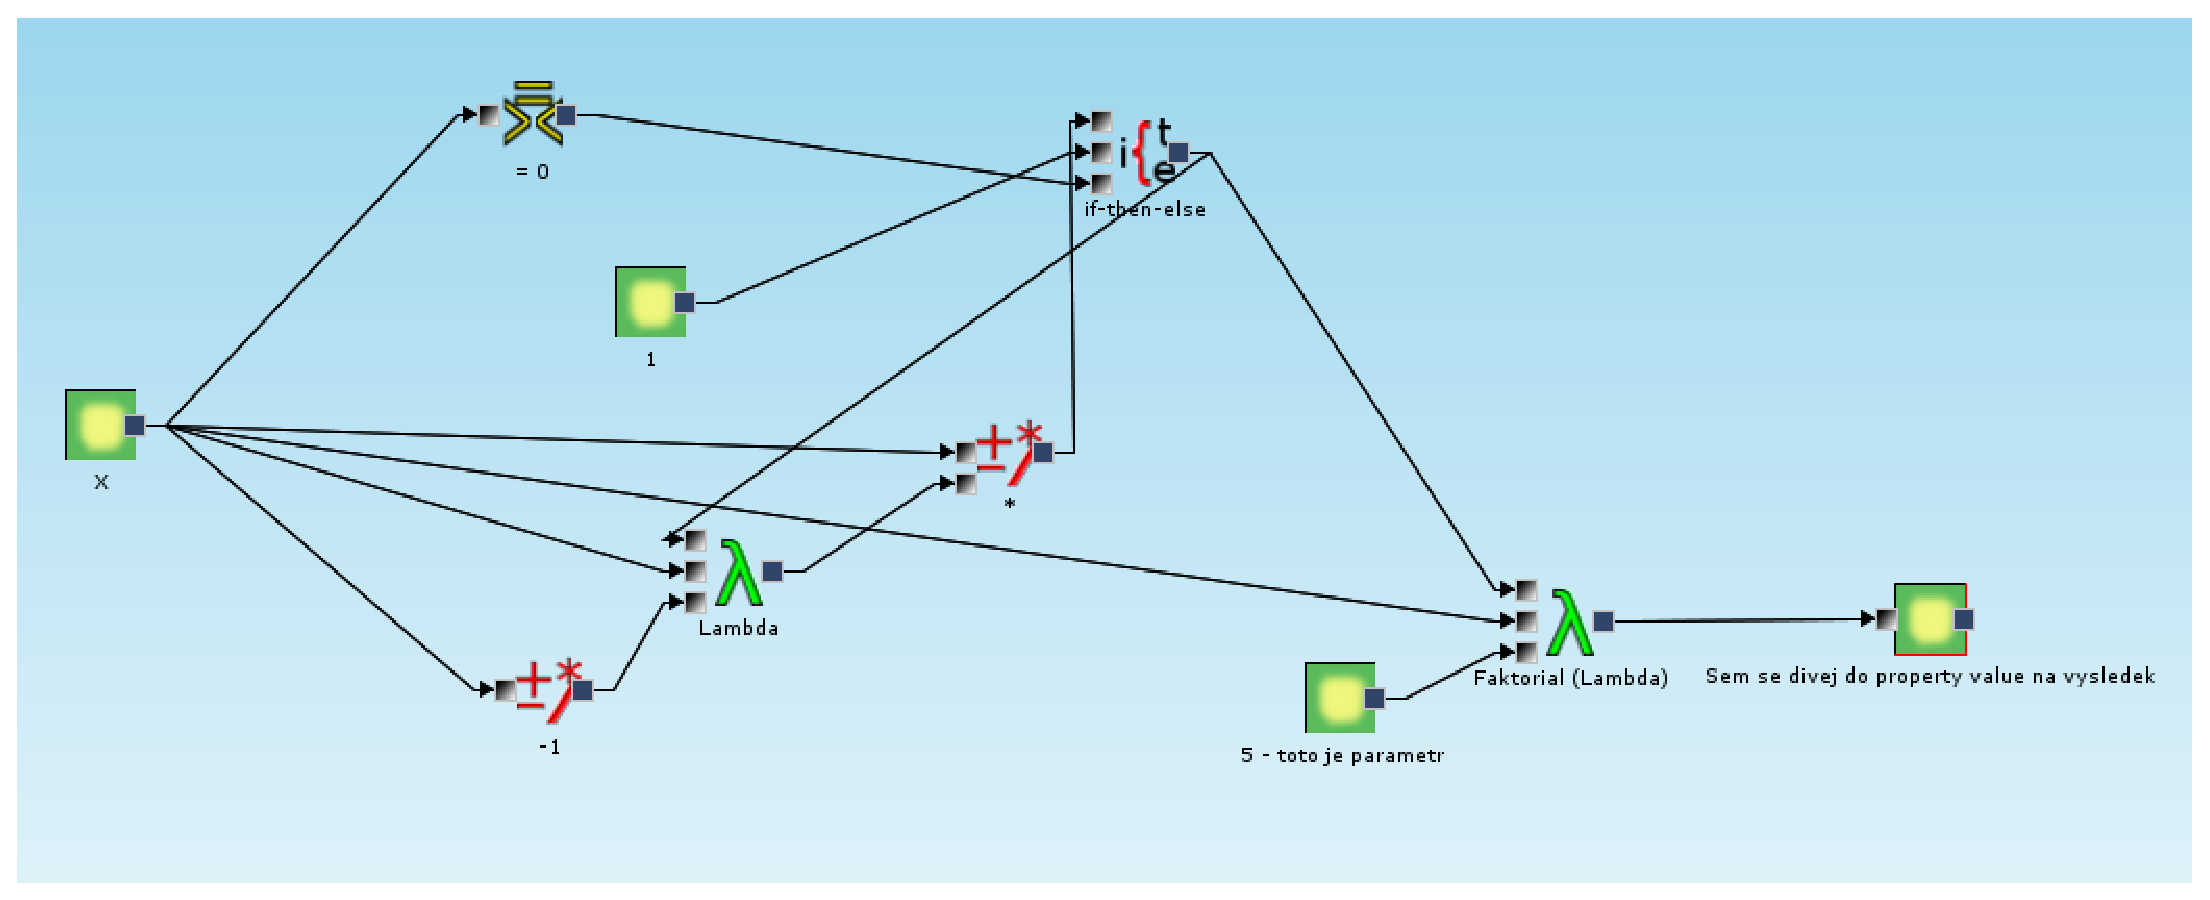
\includegraphics[width=10.8cm]{faktorial}
\end{frame}

\subsection{Other new boxes}
\begin{frame}
	\frametitle{Movie -- Get parameter}
	\movie[externalviewer]{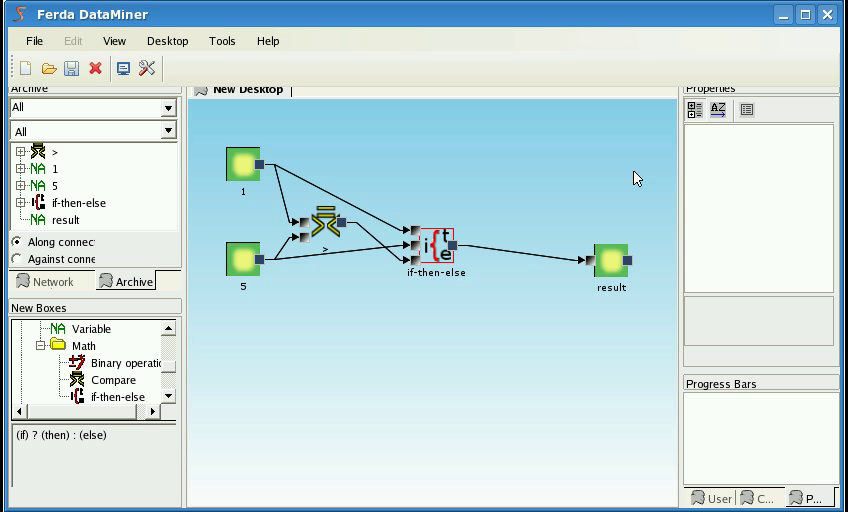
\includegraphics[width=10.8cm]{getParameter1.png}}{getParameter.ogg}
\end{frame}

\begin{frame}
	\frametitle{Get parameter}
	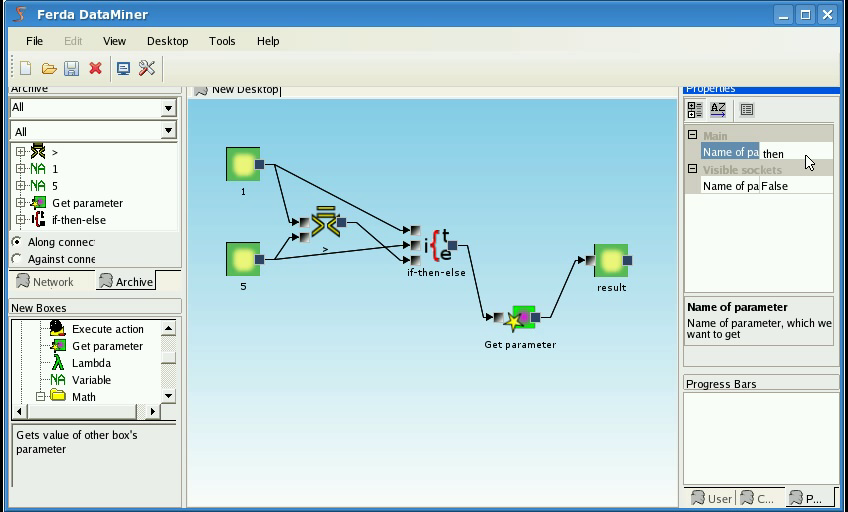
\includegraphics[width=10.8cm]{getParameter2.png}
\end{frame}

\begin{frame}
	\frametitle{Movie -- Execute action}
	\movie[externalviewer]{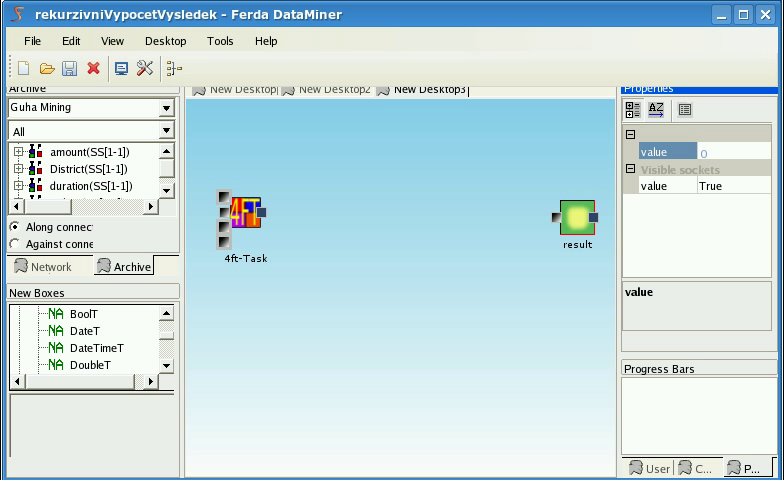
\includegraphics[width=10.8cm]{executeAction1.png}}{executeAction.ogg}
\end{frame}

\begin{frame}
	\frametitle{Execute action}
	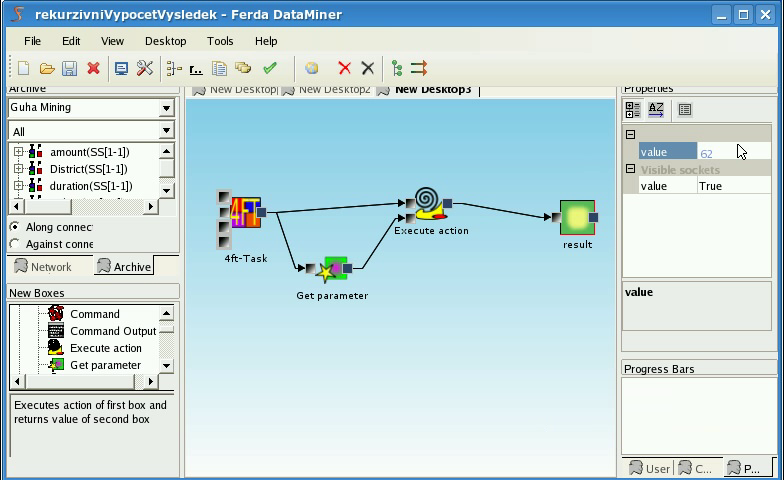
\includegraphics[width=10.8cm]{executeAction2.png}
\end{frame}

\begin{frame}
	\frametitle{Movie -- Command and command output}
	\movie[externalviewer]{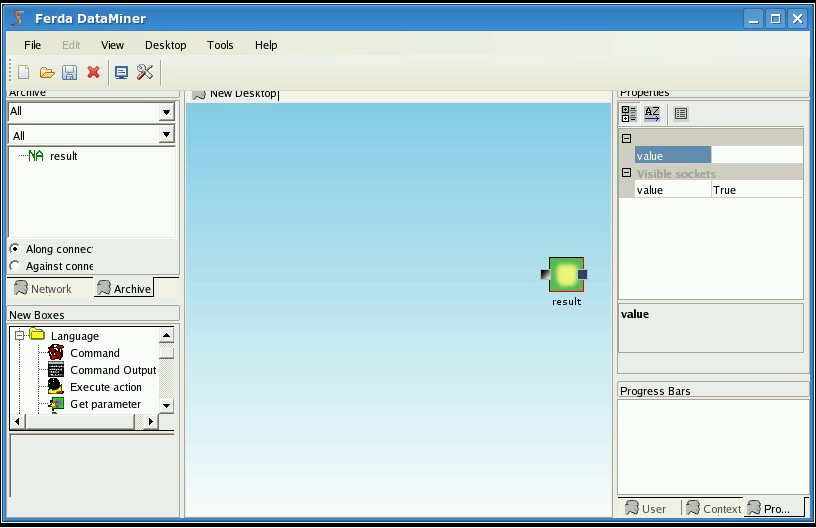
\includegraphics[width=10.8cm]{command1.png}}{command.ogg}
\end{frame}

\begin{frame}
	\frametitle{Command and command output}
	\framesubtitle{Example in ferda}
	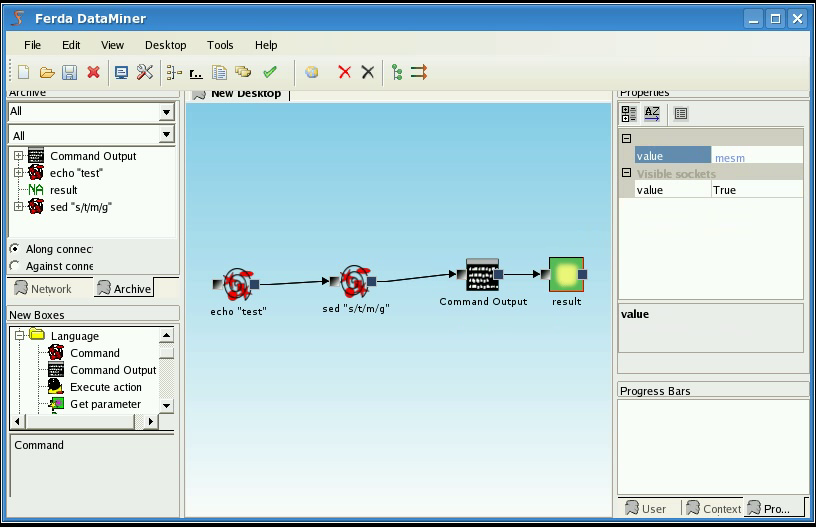
\includegraphics[width=10.5cm]{command2.png}
\end{frame}

\begin{frame}
	\frametitle{Command and command output}
	\subtitle{The same in console}
	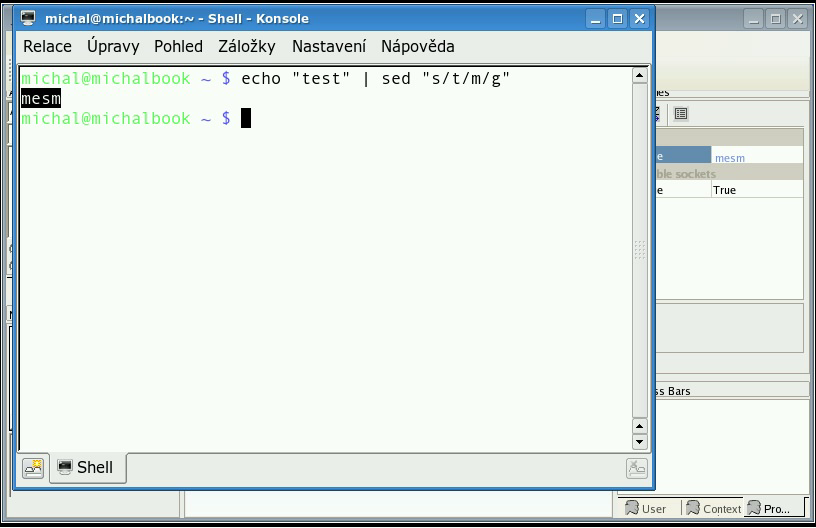
\includegraphics[width=10.8cm]{command3.png}
\end{frame}

\section{Example -- executing four fold task recursively}
\subsection{Motivation}
\begin{frame}
	\frametitle{Movie -- When lambda can be useful -- 4FT task}
	\movie[externalviewer]{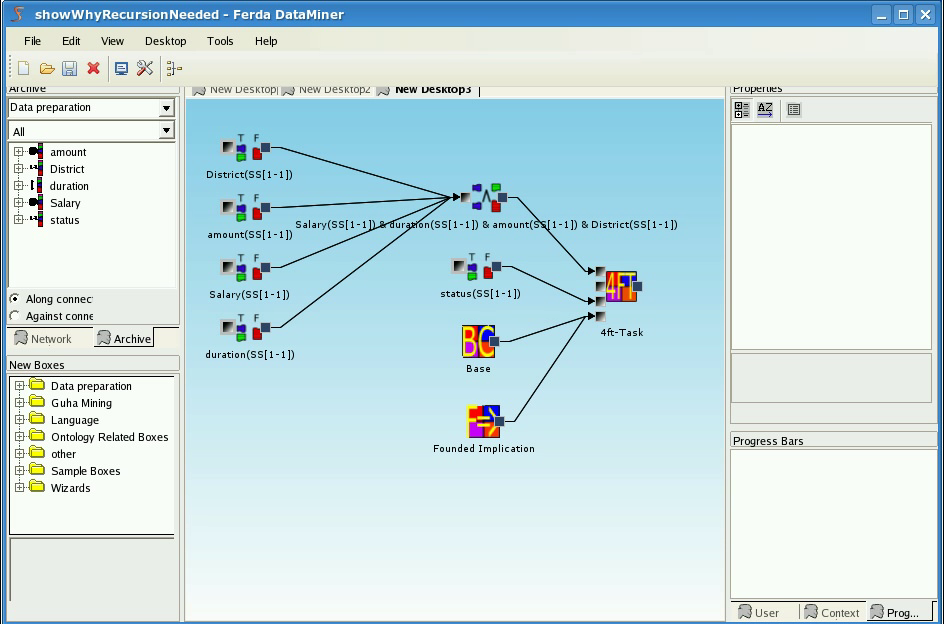
\includegraphics[width=10.8cm]{exampleMotivation1}}{exampleMotivation.ogg}
\end{frame}

\begin{frame}
	\frametitle{When lambda can be useful -- 4FT task}
	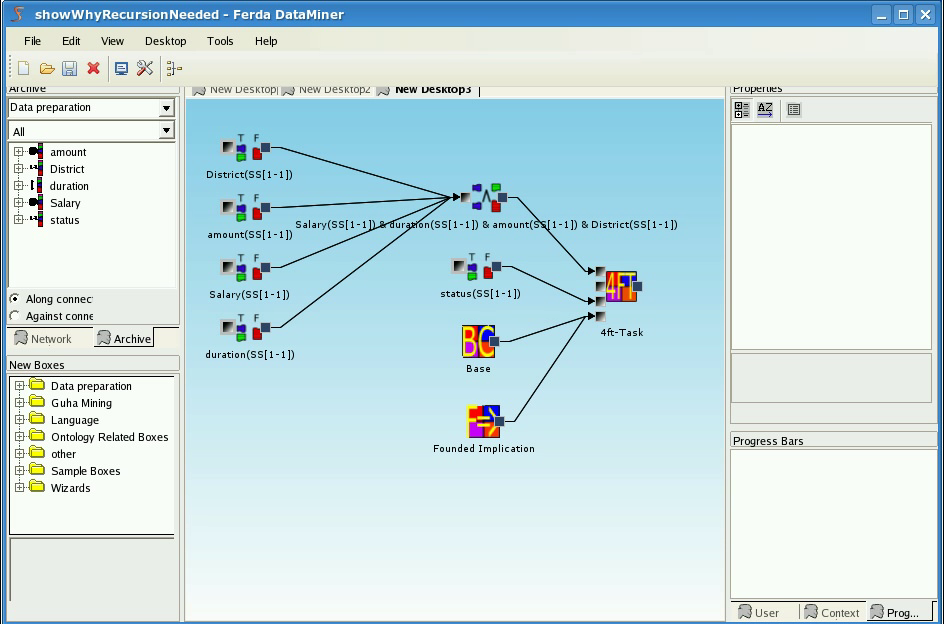
\includegraphics[width=5cm]{exampleMotivation1}
	\begin{block}<+->{Problem}
		\begin{itemize}[<+->]
			\item User tries some setting of quantifiers
			\item If he fails, he tries again with other settings?
			\item It's manual and confusing
		\end{itemize}	
	\end{block}
\end{frame}

\begin{frame}
	\frametitle{User specified automation of settings}
	\begin{block}{User wants}
		\begin{itemize}[<+->]
			\item find the best settings for task
			\item suggest way how to find best settings
			\item have for different tasks different methods
		\end{itemize}
	\end{block}
	\begin{block}<+->{Programming finding best settings by user}
		\begin{itemize}[<+->]
			\item biggest variability
		\end{itemize}
	\end{block}

\end{frame}

\subsection{Linear interpolation}
\begin{frame}
	\frametitle{Linear interpolation}
	\framesubtitle{Basics}
	
	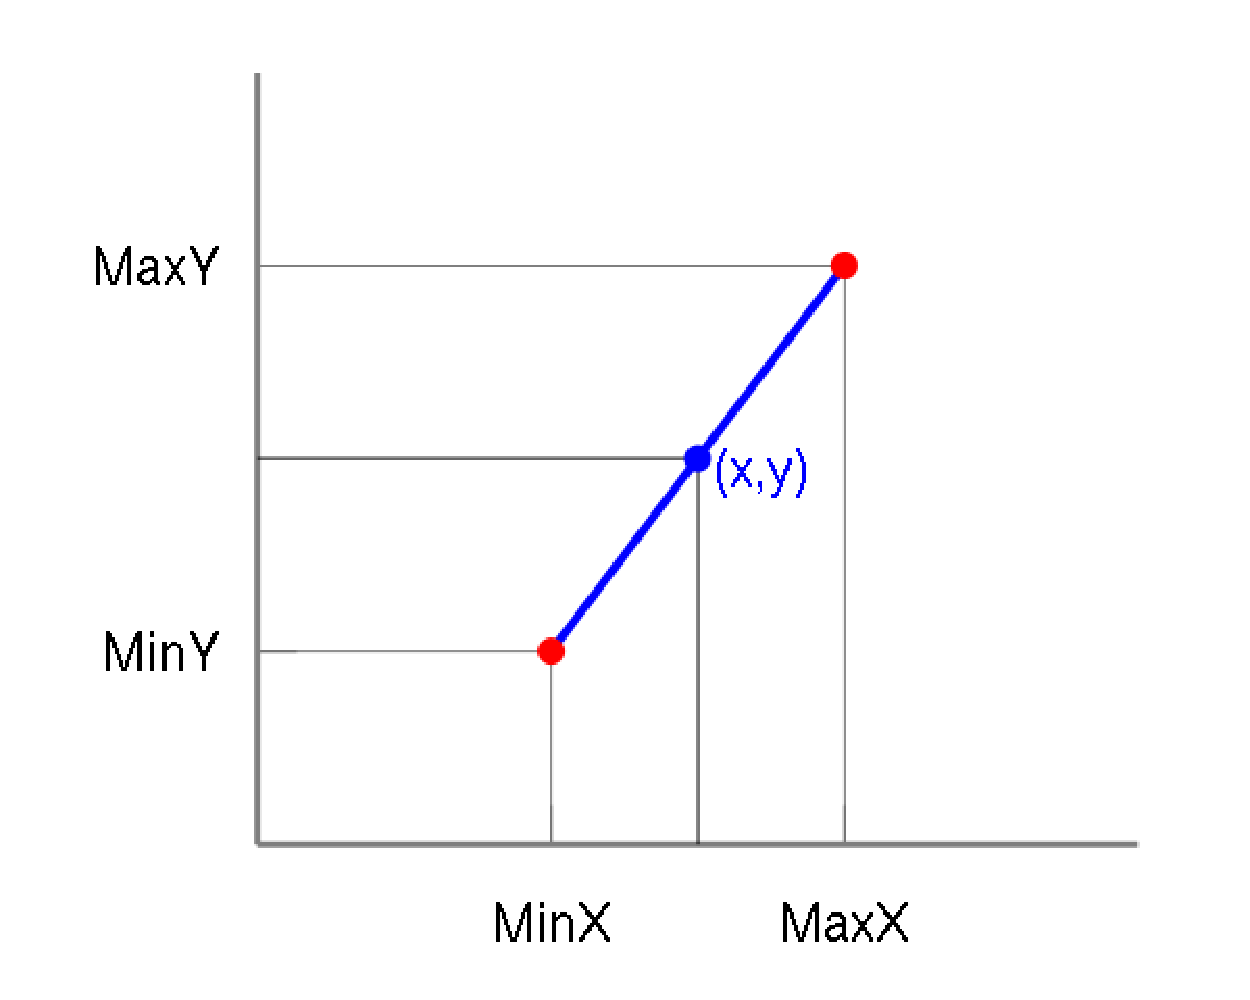
\includegraphics[width=5cm]{linearInterpolationPlot}
	\begin{block}{Formula}
		$x = MaxX - (MaxY-WantedY)\frac{MaxX - MinX}{MaxY - MinY}$
	\end{block}
\end{frame}

\begin{frame}
	\frametitle{Interpolation as connection of boxes}
	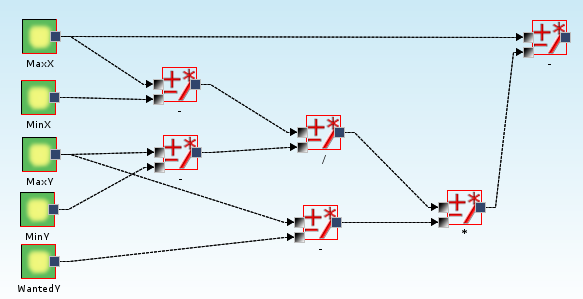
\includegraphics[width=10.8cm]{linearInterpolation}
\end{frame}

\subsection{Connection of boxes}
\begin{frame}
	\frametitle{Result should be between}
	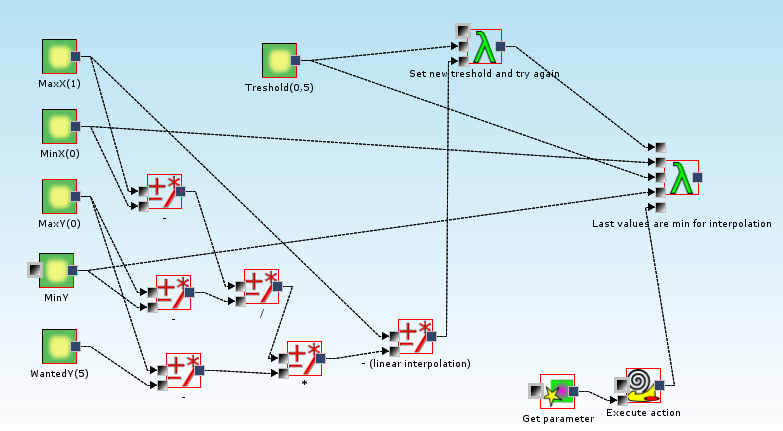
\includegraphics[width=10.8cm]{exampleMainRecursionPart}
\end{frame}

\begin{frame}
	\frametitle{If not interpolate and set new max/min}
	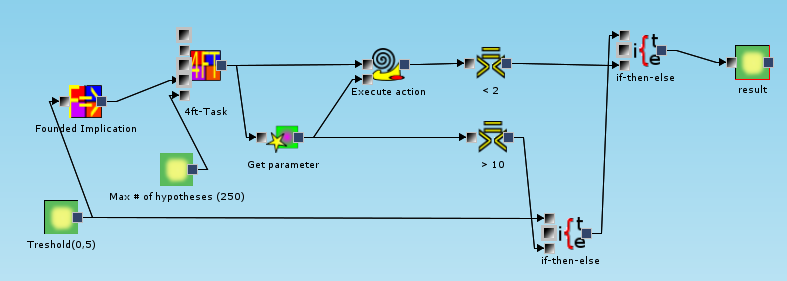
\includegraphics[width=10.8cm]{exampleMainMiningPart}
\end{frame}

\begin{frame}
	\frametitle{}
	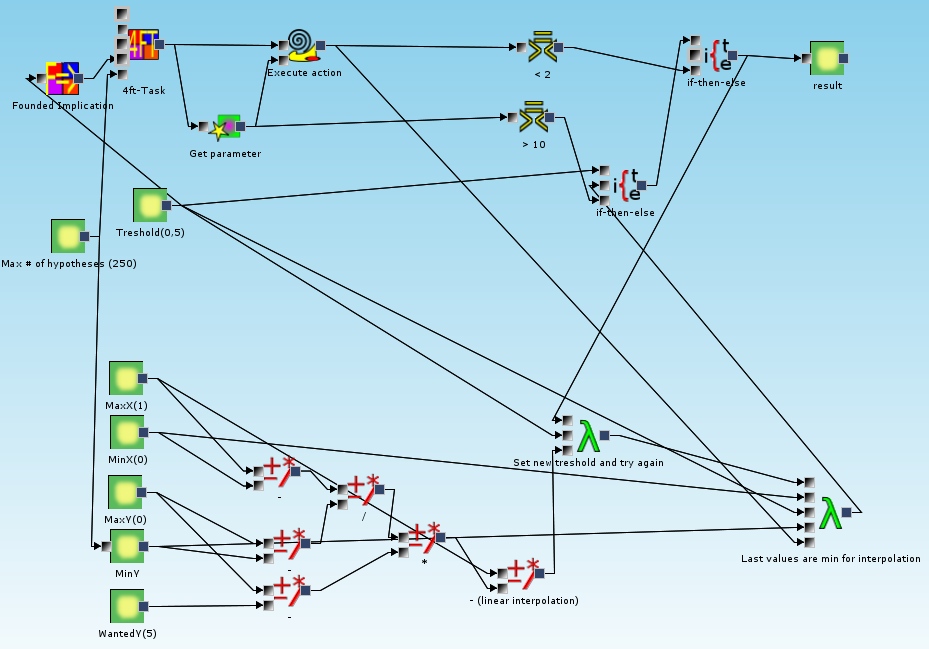
\includegraphics[width=10.8cm]{exampleWithoutInterpolationOnMax}
\end{frame}

\subsection{Results}
\begin{frame}
	\frametitle{Connection}
	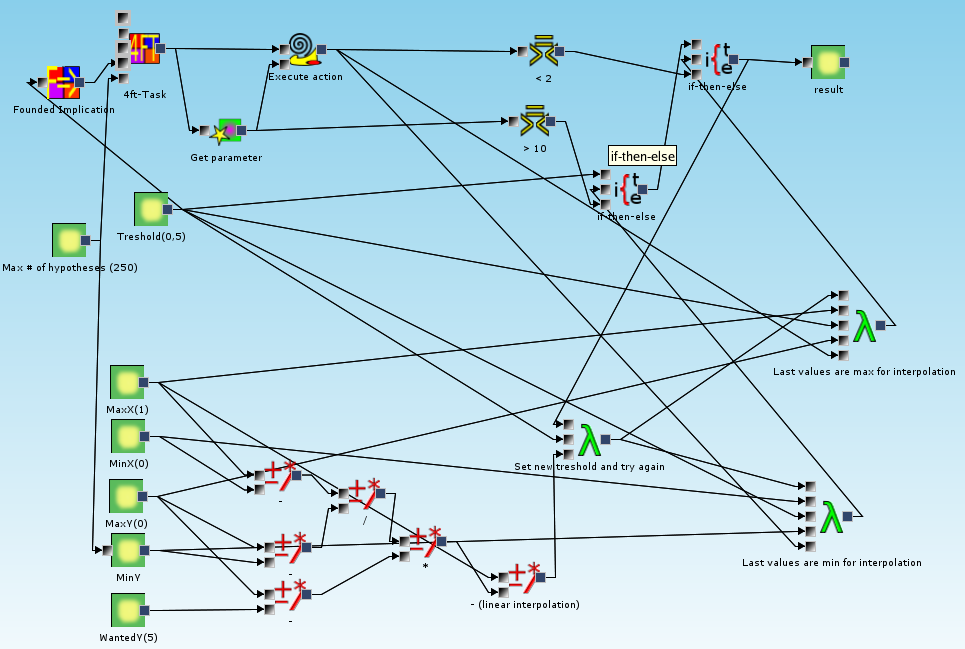
\includegraphics[width=10cm]{exampleResult}
\end{frame}

\begin{frame}
	\frametitle{Movie -- Result}
	\movie[externalviewer]{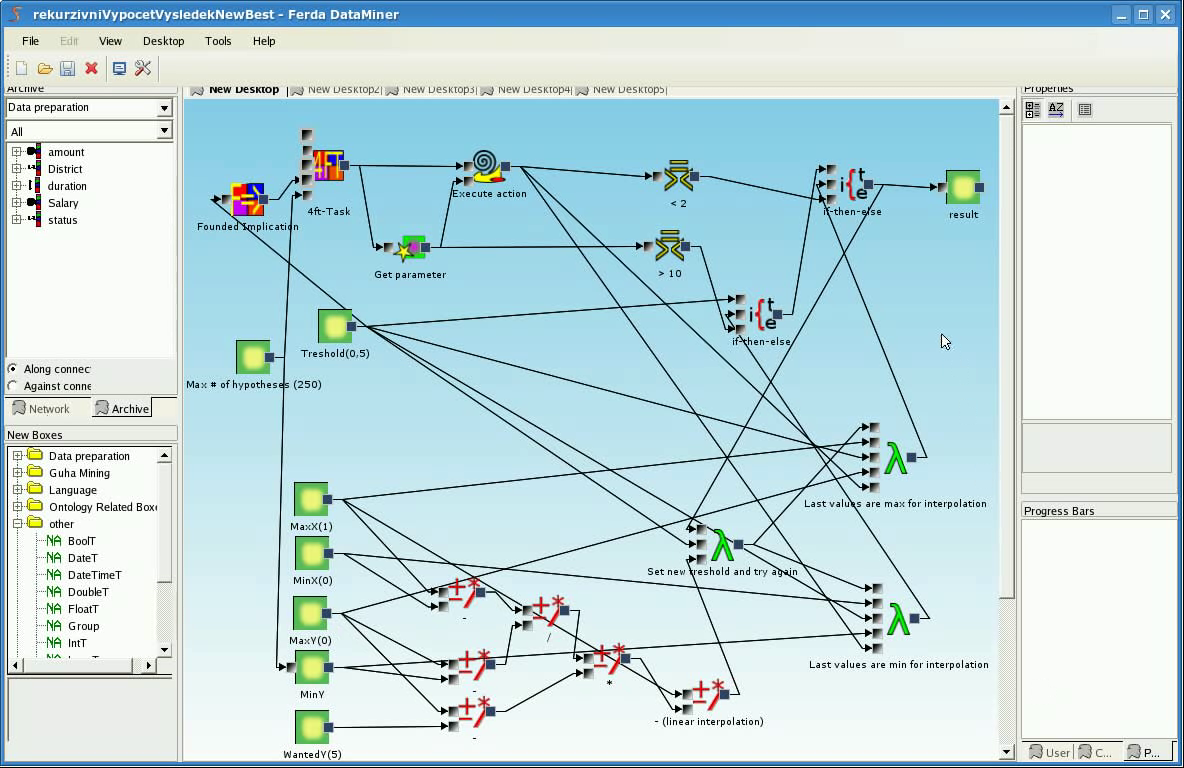
\includegraphics[width=10.8cm]{recursionExecution1}}{recursionExecution.ogg}
\end{frame}

\begin{frame}
	\frametitle{How to do it better}
	\begin{block}{Is the recursive computing of 4FT needed}
		\pause No -- BestN algorithm
	\end{block}
	\begin{block}<+->{Is user programming needed}
		\pause Yes -- even with BestN for different projects different value function
	\end{block}
\end{frame}

\section{Next steps}
\subsection{Sequences and sets}
\begin{frame}
	\frametitle{Sequences and sets}
	\begin{block}{Do we need sequences?}
		\begin{itemize}[<+->]
			\item Every mature programming language has something like sequences
			\item Sequences can be simulated, but the price
		\end{itemize}	
	\end{block}
	\begin{block}<+->{What we would like to do with sequences}
		\begin{itemize}[<+->]
			\item Make a sequence of functions
			\item Do something for each item in the sequence
			\item Add an item
			\item Subsequence
			\item Concatenation 
		\end{itemize}	
	\end{block}
\end{frame}

\begin{frame}
	\frametitle{What should be done for support of sequences?}
	\begin{block}{New boxes}
		\begin{itemize}[<+->]
			\item Sequence as head/tail
			\item Sequence as array of items
			\item ForEach
			\item AddItem, Subsequence, Concatenate
			\item New group box
			\item Box for conversion from sequence to group box
		\end{itemize}	
	\end{block}
	\begin{block}<+->{Changes to Ferda core}
		\pause Socket should accept new group box the same way it accepts the old one
	\end{block}
\end{frame}

\begin{frame}
	\frametitle{Sequence example on DM}
	\begin{block}{Problem}
		You have a table and don't know anything about.
		You would like to know something about it.
	\end{block}
	\begin{block}<+->{Resolution}
		\begin{itemize}[<+->]
			\item Connect all columns you want to analyze to the sequence
			\item Regarding types of colums and their data, create attributes for each column in the sequence
			\item Create basic tasks
			\item See result of these tasks
		\end{itemize}
	\end{block}
\end{frame}

\subsection{Reuse of code}
\begin{frame}
	\frametitle{Reuse of code}
	\framesubtitle{Problem description}
	\begin{block}{Problem}
		The user wants to reuse boxes which he created.
	\end{block}
	\begin{block}<+->{We have}
		\begin{itemize}[<+->]
			\item Project files
			\item Network archive
		\end{itemize}
	\end{block}
\end{frame}

\begin{frame}
	\frametitle{Reuse of code}
	\framesubtitle{Better network archive}
	\begin{block}{What can be done}
		\begin{itemize}[<+->]
			\item Labels
			\item More network archives
			\item User access rights
		\end{itemize}
	\end{block}
\end{frame}

\begin{frame}
	\frametitle{Reuse of code}
	\framesubtitle{Project files}
	\begin{block}{User could load boxes from other project}
		\begin{itemize}[<+->]
			\item Easy to implement
			\item There is workaround with network archive
		\end{itemize}
	\end{block}
	\begin{block}<+->{Including other project}
		\begin{itemize}[<+->]
			\item Like other programming languages
			\item Strong
			\item Harder to implement
		\end{itemize}
	\end{block}
\end{frame}

\subsection{Better lambda}
\begin{frame}
	\frametitle{Better lambda}
	\begin{block}{}
		\begin{itemize}[<+->]
			\item Parameter could be function with parameter, not only constant
			\item Lambda is slow
		\end{itemize}
	\end{block}
	\begin{block}<+->{How to make lambda quicker}
		\begin{itemize}[<+->]
			\item Quicker creating of boxes
			\item Functions could be called only once
			\item Boxes could be clonned only in time it is really needed
		\end{itemize}
	\end{block}
\end{frame}

\subsection{Summary}
\begin{frame}
	\frametitle{Other things to do}
	\begin{block}{}
		\begin{itemize}[<+->]
			\item Most of modules for interacionts should work on top of functions not boxes
			\item Boxes for GUHA -- parts 
			\item User could choose on which computer a box is running
			\item Box which can be programmed by user at runtime in some scripting language
		\end{itemize}
	\end{block}
\end{frame}

\begin{frame}
	\frametitle{Summary}
	\begin{block}{Programming language in Ferda should}
		\begin{itemize}[<+->]
			\item offer more power for data mining
			\item allow to do things which were not designed before
		\end{itemize}
	\end{block}
	\begin{block}<+->{Next steps}
		\begin{itemize}[<+->]
			\item there are many things to do
		\end{itemize}
	\end{block}
\end{frame}

\end{document}
